\documentclass[a4paper,12pt]{article}

% Packages
\usepackage{graphicx}
\usepackage{amsmath}
\usepackage{geometry}
\usepackage{fancyhdr}
\usepackage{setspace}
\usepackage{subcaption}
\usepackage{titlesec}  % For title formatting
\geometry{margin=1in}
\usepackage[utf8]{inputenc}
\usepackage{polski}
\usepackage{hyperref}
\usepackage{algpseudocode}
\usepackage{float}
\usepackage{dsfont}
\setstretch{1.2}

\DeclareMathOperator*{\argmin}{arg\,min}

% Header and Footer
\pagestyle{fancy}
\fancyhf{}
\fancyhead[L]{Klasyfikacja binarna ciąg dalszy}
\fancyhead[R]{\thepage}

% Title Formatting
\titleformat{\section}{\normalfont\Large\bfseries}{\thesection}{1em}{}

% Cover Page
\title{
    \vspace{2cm} % Adjust vertical space
    \begin{figure}[h!]
        \centering
        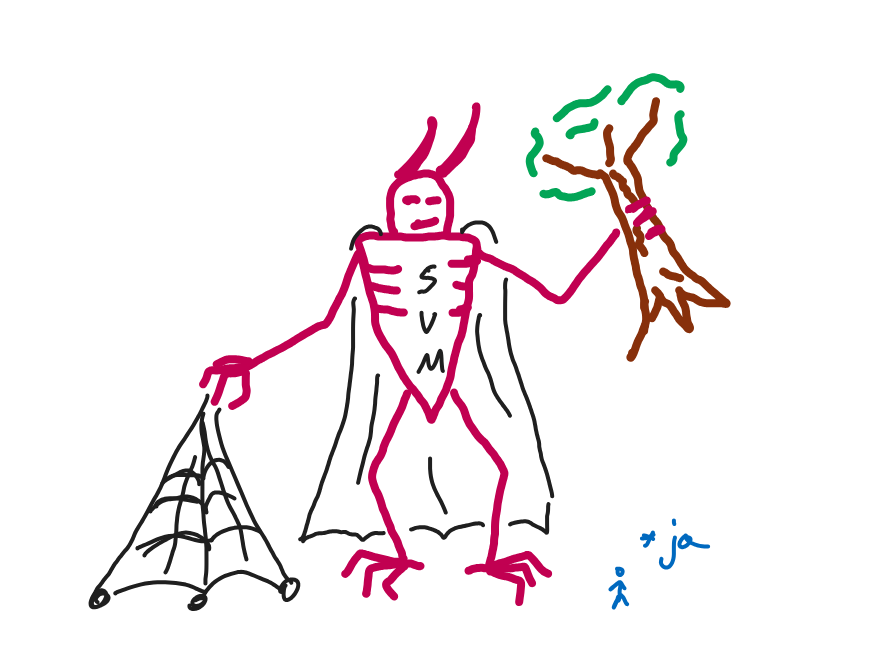
\includegraphics[width=0.8\textwidth]{title.png} 
        \caption{Evil SVM}
    \end{figure}
    \vspace{1cm} % Adjust vertical space after the logo
    \textbf{\Huge Miniprojekt 2: Klasyfikacja binarna ciąg dalszy} \\
    \vspace{1cm} % Adjust vertical space
    \large Metody Probabilistyczne w Uczeniu Maszynowym \\
    \vspace{0.5cm} % Adjust vertical space
    \large \date{\today}
}
\author{Szymon Szulc}


\begin{document}

% Title Page
\maketitle
\thispagestyle{empty}
\newpage

% Table of Contents
% Start page numbering from the Table of Contents
\setcounter{page}{1}  % Start counting from 1
\tableofcontents
\newpage

\section{Wstęp}
Niniejszy raport oparty jest na notatnikach \texttt{*.ipynb}. Raport ma stanowić zwięzłe i czytelne podsumowanie mojej pracy nad problemem klasyfikacji binarnej korzystając z maszyny wektorów nośnych, głebokiej sieci neuronowej oraz drzewa decyzyjnego.

\section{Badany problem}
\subsection{Definicja}
Dane na jakich pracujemy to jakieś cechy stron internetowych. Naszym zadaniem jest stwierdzić, czy strona internetowa służy do phishingu (1), czy też jest bezpieczna (-1).
\subsection{Założenia}
Formalnie:
\begin{align*}
    &y \in \{-1, 1\} \\
    &\forall i \in \{0,\dots,20\} \hspace{7pt} x_i \in \{-1, 1\} \\
    &\forall j \in \{21,\dots,28\} \hspace{7pt} x_j \in \{-1, 0, 1\} \\
    & x_{29} \in \{0, 1\} \\
\end{align*}
Mamy do czynienia z cechami dyskretnymi. Nie wiemy nic o ich rozkładach.

\section{Pierwszy kontakt z danymi}
Mamy 30 cech -- $x_0, \dots, x_{29}$ i zmienną binarną $y$. Żeby podtrzymać tradycję, patrzymy na \hyperref[fig:corr]{macierz korelacji}, którą już bardzo dobrze znamy i przynajmniej empirycznie wiemy, że nie odbiega bardzo od testu chi-kwadrat.

\begin{figure}[H]
    \centering
    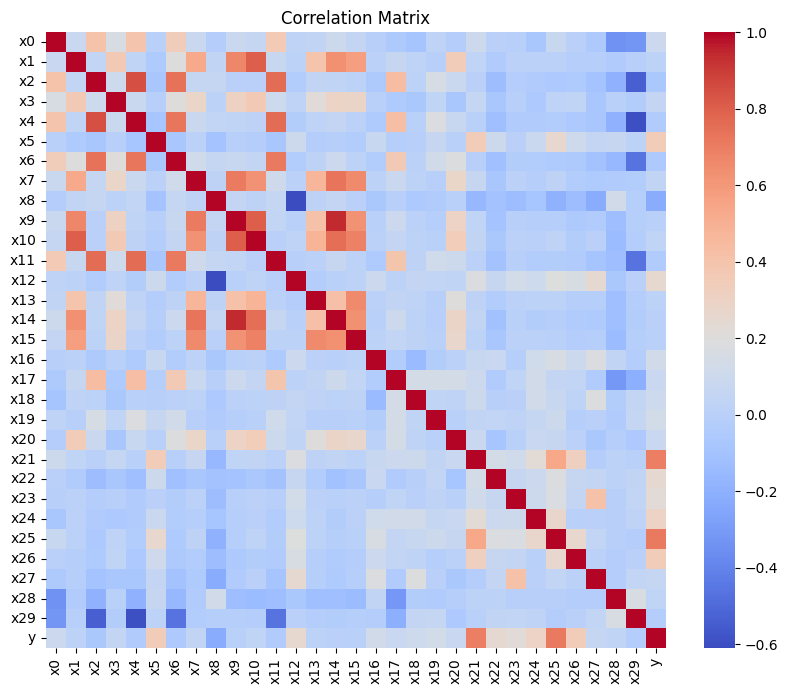
\includegraphics[width=0.8\textwidth]{corr.png} 
    \caption{Macierz korelacji Pearsona}
    \label{fig:corr}
\end{figure}

\!\!\!\!\!\!\!\!\!Możemy zauważyć, że silnie skorelowanych jest tylko kilka cech. Wydaje się, że moglibyśmy się ich pozbyć bez straty na dokładności modelu. Ta hipoteza potwierdziła się dopiero przy drzewach decyzyjnych.

\section{Podział danych}
Dokonałem losowego podziału danych (60\% -- zbiór treningowy, 20\% zbiór walidacyjny, 20\% zbiór testowy, zachowując również taki stosunek w obrębie klas $y$) 10 razy, żeby uśrednić wyniki.

\section{Maszyna wektorów nośnych (SVM)}
\subsection{Wstęp}
Będę korzystał z wariantu z regularyzacją.
\begin{align*}
    &\text{Chcemy zminimalizować} && \frac{1}{2} \|w\|^2 + C \sum_{i=1}^m \xi_i \\
    &\text{pod warunkiem} && y^{(i)} \left( w^T x^{(i)} + b \right) \geq 1 - \xi_i, \quad i = 1, \ldots, m, \\
    & && \xi_i \geq 0, \quad i = 1, \ldots, m.
\end{align*}
Od razu przeszedłem na problem dualny z mnożnikami Lagrange'a $\alpha$
\begin{align*}
\min_{\alpha} \Psi(\alpha) &= \min_{\alpha} \frac{1}{2} \sum_{i=1}^m \sum_{j=1}^m y^{(i)} y^{(j)} K(x^{(i)}, x^{(j)}) \alpha_i \alpha_j - \sum_{i=1}^m \alpha_i \\
0 &\leq \alpha_i \leq C, \quad \forall i \in \{1,\dots,m\} \\
&\sum_{i=1}^m y^{(i)} \alpha_i = 0.
\end{align*}
Margines dla punktu $x$ jesteśmy w stanie policzyć bez liczenia $w$ bezpośrednio ze wzoru
\[
u = \sum_{i=1}^m y^{(i)}\alpha_i K(x^{(i)}, x) - b.
\]
Żeby wytrenować model będę korzystał z algorytmu sekwencyjnej minimalnej optymalizacji. Ale zanim przejdziemy do mojej historii o trenowaniu SVM to jeszcze słowo jak odzyskujemy $b$.
Zmienną $b$ aktualizujemy na bieżąco zgodnie z artykułem Johna C. Platta \textit{Sequential Minimal Optimization:
A Fast Algorithm for Training Support Vector Machines}. W każdym obiecującym wyborze $\alpha_1, \alpha_2$
\begin{align*}
    &b_1 = u_1 - y^{(1)} + y^{(1)}(\alpha_1^{\mathrm{new}} - \alpha_1)K(x^{(1)}, x^{(1)}) + y^{(2)}(\alpha_2^{\mathrm{new,clipped}} - \alpha_2)K(x^{(1)}, x^{(2)}) + b \\ 
    &b_2 = u_2 - y^{(2)} + y^{(1)}(\alpha_1^{\mathrm{new}} - \alpha_1)K(x^{(1)}, x^{(2)}) + y^{(2)}(\alpha_2^{\mathrm{new,clipped}} - \alpha_2)K(x^{(2)}, x^{(2)}) + b \\ 
    &b^{\mathrm{new}} = \frac{b_1 + b_2}{2}.
\end{align*}
Nie musimy zatem odzyskiwać $b$, ponieważ zawsze je znamy :). \\
Żeby zwrócić predykcję $y$ wystarczy $\texttt{sign}(u)$.

\subsection{Implementacja}
Jak wyglądała moja podróż przez piekło SVMa:
\begin{enumerate}
    \item {
    Dzielnie przeczytałem artykuł i przepisałem ze zrozumieniem pseudokod, o zgrozo z użyciem pętli \texttt{for}. Tego nie dało się wytrenować. Po 2 godzinach mielenia danych nie było widać końca.
    }
    \item {
    Wprowadziłem maksymalną liczbę epok i pozbyłem się z kodu wszystkich warunków, które uważałem za niezrozumiałe -- na przykład, jeśli $\eta \leq 0$ to nie próbuję tego ratować -- zawsze możemy wybrać inne $\alpha_1, \alpha_2$ ;). Udało się wytrenować SVMa, ale teraz predykcja trwała dłużej niż trening.
    }
    \item {
    Wektoryzacja jąder. Tutaj spędziłem tylko chwilę z \texttt{numpy}. Udało się, mam wynik
    \begin{flalign*}
        &\texttt{SVM accuracy: } 0.5109 &&
    \end{flalign*}
    }
    \item {
    Załamałem się, użyłem wszystkich heurystyk wyboru $i_1, i_2$ z artykułu. Nawet wprowadziłem \texttt{error\_cache}, żeby móc uczyć przez więcej epok. Wszystko na nic, również dobrze mógłbym rzucać monetą w czasie stałym.
    }
    \item {
    Oświecenie. Źle liczyłem samą predykcję, funkcja \texttt{np.nonzero} (która miała na celu optymalizację -- zwracała indeksy $\alpha_i \neq 0$ -- wektory nośne, których było zazwyczaj $\approx 900$ -- znacznie mniej niż wielkość zbioru danych) jest bardzo podła i zwraca coś czego byśmy się nie spodziewali. Do podmianie na \texttt{np.argwhere} w końcu można zabrać się za dobieranie hiperparametrów.
    }
\end{enumerate}
\subsection{Hiperparametry i jądra}
Zaznaczę, że przy SVMach nie stosuję standaryzacji cech. \\ 
Zaczynamy od jądra liniowego -- zwykłego iloczynu skalarnego. Od tego momentu błąd to znany błąd zero-jedynkowy.
\begin{flalign*}
&\texttt{Average validation error for SVM SMO with C=5.0: } 0.1372 && \\
&\texttt{Average validation error for SVM SMO with C=1.0: } 0.1304 && \\
&\texttt{Average validation error for SVM SMO with C=0.1: } 0.1373 && \\
&\texttt{Average validation error for SVM SMO with C=0.01: } 0.1373 &&
\end{flalign*}
Jak widać $C=1$ tworzy lokalne minimum. Trenowałem model przez 5000 epok. Zajęło to 4.8s. Dało przyzwoity wynik.
\begin{flalign*}
&\texttt{Average test accuracy for SVM SMO with C=1.0: } 0.8680 &&
\end{flalign*}
\begin{figure}[H]
    \centering
    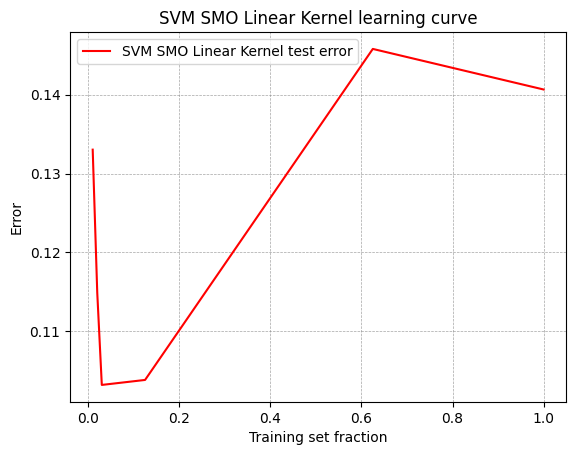
\includegraphics[width=0.75\textwidth]{svm_linear.png}
    \caption{Krzywa uczenia SVMa z liniowym jądrem}
    \label{fig:svm-lin}
\end{figure}
\!\!\!\!\!\!\!\!\!Ten \hyperref[fig:svm-lin]{wykres} wygląda co najmniej dziwnie. Być może jest to wina doborów $\alpha_1, \alpha_2$ lub zmiany wektorów nośnych.

\vspace{22pt}

\!\!\!\!\!\!\!\!\!Teraz jądro gaussowskie. Oczekujemy, że wynik się poprawi, a czas nauki wydłuży, ponieważ liczenie \texttt{exp} jest kosztowne. Zostawiłem $C=1$, a walidacja wskazała $\sigma=7$.
\begin{flalign*}
&\texttt{Average validation error for SVM SMO with Gaussian kernel sigma=0.1: } 0.4370 && \\
&\texttt{Average validation error for SVM SMO with Gaussian kernel sigma=1: }   0.3433 && \\
&\texttt{Average validation error for SVM SMO with Gaussian kernel sigma=7: }   0.1297 && \\
&\texttt{Average validation error for SVM SMO with Gaussian kernel sigma=14: }  0.1990 &&
\end{flalign*}
Czas nauki dla 5000 epok wyniósł 18.2s -- 4 razy dłużej. Wyniki nie są dużo lepsze, być może dane były prawie liniowo separowalne.
\begin{flalign*}
&\texttt{Average test accuracy for SVM SMO with Gaussian kernel sigma=7: } 0.9091 && 
\end{flalign*}
Natomiast mam wrażenie, że samo uczenie przebiega bardziej gładko co widać na \hyperref[fig:svm-ker]{wykresie}.

\begin{figure}[H]
    \centering
    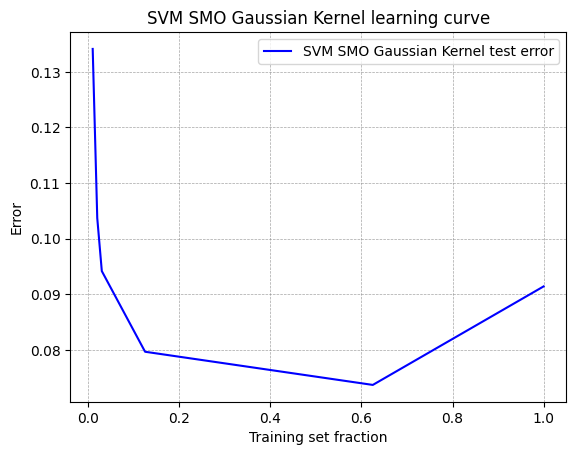
\includegraphics[width=0.75\textwidth]{svm_kernel.png}
    \caption{Krzywa uczenia SVMa z gaussowskim jądrem}
    \label{fig:svm-ker}
\end{figure}

\begin{figure}[H]
    \centering
    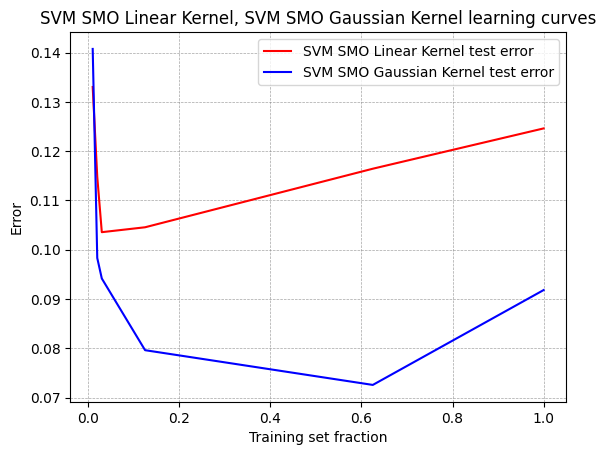
\includegraphics[width=0.75\textwidth]{svm_comp.png}
    \caption{Krzywe uczenia SVMów}
    \label{fig:svm-comp}
\end{figure}

\newpage

\section{Drzewo decyzyjne a miał być las}
\subsection{Wstęp}
Drzewa decyzyjne są bardzo intuicyjne i powinny dawać bardzo dobre rezultaty dla zbioru treningowego. One po prostu dzielą przestrzeń na podstawie najlepszych cech i podprzestrzeniom nadają etykiety zgodnie z głosem większości próbek w danej podprzestrzeni. 
\subsection{Implementacja}
Ja do sprawdzania, jak dobry jest podział, użyłem klasycznej miary -- \texttt{Gini Impurity}. Implementacja obyła się bez jakichkolwiek problemów. Przeszukujemy dany podzbiór (tak, podzbiór bo w zamyśle chciałem mieć gotową implementację pod las, a dla drzew przekazywać cały zbiór cech zawsze) cech, wybieramy najlepszą i rekursja. Podkradłem ujmującą sztuczkę z kanału na YouTube StatQuest -- możemy posortować unikalne wartości danej cechy i sprawdzać podziały ze względu na średnią 2 sąsiednich elementów. To nam załatwia cechy binarne i resztę bez ifowania. Jako hiperparametr wprowadziłem \texttt{max\_depth}, żeby ograniczyć przeuczenie.

\subsection{Wielkie odkrycie}
Wytrenowałem drzewo z $\texttt{max\_depth}=8$, żeby zobaczyć czy wszystko działa.
\begin{flalign*}
&\texttt{Validation error fot DT: } 0.0644 && 
\end{flalign*}
Ja nie dowierzałem. Oczekiwałem, że będzie źle. Wytrenowałem drzewo o głebokości 1 -- to jest dokładnie 1 podział.
\begin{flalign*}
&\texttt{Validation error fot DT: } 0.1111 && 
\end{flalign*}
Co więcej to była cecha $x_{25}$ -- przywołując \hyperref[fig:corr]{macierz korelacji} -- cecha o najwyższym współczynniku Pearsona. Dopiero teraz zdałem sobie sprawę jak bardzo mogłem przyspieszyć SVMa. Wystarczyło usunąć nieistotne cechy. Taki wynik drzewa decyzyjnego potwierdza nam również, że dane są prawie liniowo separowalne -- przynajmniej tak mi się wydaje.

\subsection{Hiperparametry}
\begin{flalign*}
&\texttt{Average validation error for DT with max\_depth=1: }  0.1111 && \\
&\texttt{Average validation error for DT with max\_depth=8: }  0.0644 && \\
&\texttt{Average validation error for DT with max\_depth=16: } 0.0438 &&
\end{flalign*}
Pewnie moglibyśmy zejść z błędem jeszcze niżej, ale trenowanie trwało już zbyt długo, pętle \texttt{for} są bardzo niewydajne.
Ostatecznie drzewo decyzyjne z maksymalną głębokością 16 trenowało się 18.5s. Osiągnęło świetny wynik.
\begin{flalign*}
&\texttt{Average test accuracy for DT with max\_depth=16: } 0.9533 &&
\end{flalign*}
Podzieliło przestrzeń na 363 podprzestrzenie -- być może bym to jakoś skomentował, jeśli obejrzałbym wykład 10., który zdaje się być o wymiarze Vapnika. Trenowało się bardzo \hyperref[fig:tree]{gładko}.

\begin{figure}[H]
    \centering
    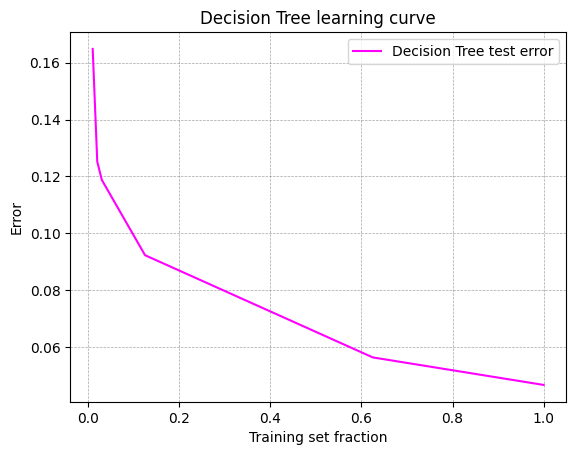
\includegraphics[width=0.75\textwidth]{tree.png}
    \caption{Krzywa uczenia drzewa decyzyjnego}
    \label{fig:tree}
\end{figure}

\section{Głęboka sieć neuronowa}
\subsection{Wstęp}
Plany były bardzo ambitne. Chciałem pobawić się z różnymi metodami schodzenia gradientem: SGD, Nesterov, Adam. Niestety piekielny SVM pokrzyżował moje plany. Skończyło się na następującej architekturze:
\[
\begin{array}{l}
\text{Warstwa 1:} \quad \text{input\_dim} = 30, \quad \text{output\_dim} = 32 \\
\text{Warstwa 2:} \quad \text{input\_dim} = 32, \quad \text{output\_dim} = 16 \\
\text{Warstwa 3:} \quad \text{input\_dim} = 16, \quad \text{output\_dim} = 1 \\
\text{Na końcu: } \quad \text{funkcja aktywacji } \texttt{sigmoid}
\end{array}
\]
Ta architektura nie ma większego uzasadnienia. Bierzemy liczbę cech i tak stopniowo zmniejszamy aż do 1.
Ponadto dla każdej warstwy są wyrazy wolne, wagi inicjalizuję metodą \texttt{He} -- mam już doświadczenie, że bez tego gradient eksploduje. Gradient to zwykły \texttt{SGD} z \texttt{batch\_size} i stałym \texttt{learning\_rate}. Jako funkcję aktywacji używam \texttt{ReLU}, a funkcja straty to znana binarna entropia krzyżowa.

\subsection{Implementacja}
Jedyną trudnością jest tutaj propagacja wsteczna. Trzeba chwilę pogłówkować jak użyć tam \texttt{numpy}.

\subsection{Hiperparametry}
Ostatecznie skończyło się na $\texttt{batch\_size}=512$, $\texttt{epochs}=100$, $\texttt{learning\_rate}=0.01$.
Bardzo lubię oglądać wykresy training error vs epoch, więc taki też \hyperref[fig:nn-gd]{przygotowałem}. To pokazuje jakie problemy ma optymalizator, żeby wbić się w minimum. Lepsze optymalizatory byłyby gładsze.

\begin{figure}[H]
    \centering
    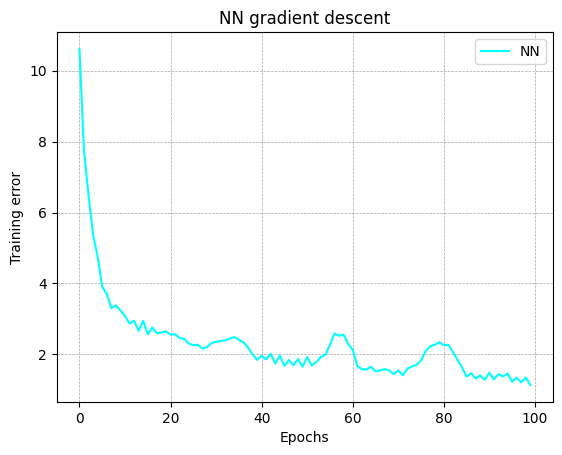
\includegraphics[width=0.75\textwidth]{nn_gd.png}
    \caption{Spadek gradientowy}
    \label{fig:nn-gd}
\end{figure}

\!\!\!\!\!\!\!\!\!Jak można było się spodziewać, taka prosta sieć średnio sobie radzi, ma trudności z zejściem do minimum, być może schodzi do złego minimum.

\begin{flalign*}
&\texttt{Average accuracy for NN: } 0.8063 && 
\end{flalign*}

\begin{figure}[H]
    \centering
    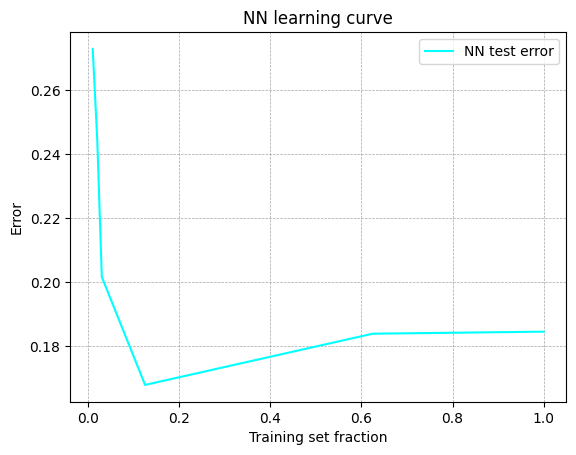
\includegraphics[width=0.75\textwidth]{nn.png}
    \caption{Krzywe uczenia NN}
    \label{fig:nn}
\end{figure}

\newpage 

\section{Porównanie}
Absolutnie nie spodziewałem się takiego wyniku. Szczerze liczyłem, że piękna matematyka, która stoi za SVM zwycięży, jednak okazała się bardzo trudna do implementacji. Najprostsze drzewo decyzyjne okazało się najlepsze w wykrywaniu czy strona służy do phishingu.

\begin{figure}[H]
    \centering
    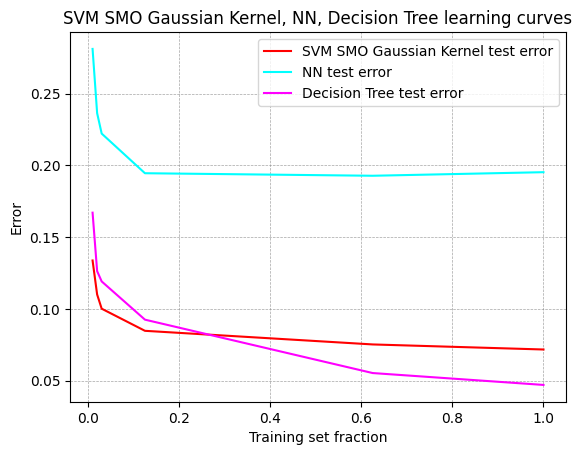
\includegraphics[width=0.75\textwidth]{comp.png}
    \caption{Wszystkie krzywe uczenia}
    \label{fig:comp}
\end{figure}

\section{Podsumowanie}
Ten miniprojekt nauczył mnie wiele. Po pierwsze nie ufać nazwom funkcji. Do drugie pętla \texttt{for} jest bardzo wolna w \texttt{Pythonie}. Po trzecie i najważniejsze warto sprawdzić kilka modeli dla 1 problemu, możemy na przykład odkryć, że dane są prawie liniowo separowalne przez 1 cechę.

% Bibliography (if required)
% \bibliographystyle{plain}
% \bibliography{references}  % Add a .bib file if you have references

\end{document}